\documentclass[conference]{IEEEtran}
\usepackage{cite}
\usepackage{amsmath,amssymb,amsfonts}
\usepackage{algorithmic}
\usepackage{graphicx}
\usepackage{textcomp}
\usepackage{xcolor}
\def\BibTeX{{\rm B\kern-.05em{\sc i\kern-.025em b}\kern-.08em
    T\kern-.1667em\lower.7ex\hbox{E}\kern-.125emX}}

\begin{document}
\title{Survey on Aspect-Based Sentiment Analysis}

\author{\IEEEauthorblockN{Mohammad Ahmad}
\IEEEauthorblockA{\textit{CS Department - Harrisburg Campus}\\
\textit{Pennsylvania State University}\\
Middletown, USA\\
mohammad.ahmad@psu.edu}
}

\maketitle
\thispagestyle{plain}
\pagestyle{plain}

\begin{abstract}
This document is a model and instructions for \LaTeX.
This and the IEEEtran.cls file define the components of your paper [title, text, heads, etc.]. *CRITICAL: Do Not Use Symbols, Special Characters, Footnotes, 
or Math in Paper Title or Abstract.
\end{abstract}

\begin{IEEEkeywords}
component, formatting, style, styling, insert
\end{IEEEkeywords}

\section{Introduction}
An important area of study within the field of Natural Language Processing (NLP) is Sentiment Analysis (SA). SA is defined as extracting the emotional tone or the expressed polarity in a given text. This is usually done by classifying a given text as expressing a positive, a negative, or a neutral sentiment. A further area of study within SA is Feature-Based or Aspect-Based Sentiment Analysis (ABSA). This refers to the extraction of expressed sentiments about the individual entities or objects within a text.

The motivation behind studying ABSA is simply that there is no scarcity in the amount of text containing opinions being produced. And it is often too simplistic of an approach to deem an entire text as expressing a positive, a negative, or a neutral opinion. The reality is that within an opinion piece, the writer is usually expressing opinions regarding multiple different aspects or subjects which then build up to the overall opinion being expressed by the text. Though it is valuable to find out the overall opinion being expressed by a text, it is more actionable for a concerned entity of an opinion piece to be able to extract the opinions about the individual aspects mentioned within the text.

Two important subtasks in ABSA are Aspect Extraction (AE) and Aspect Sentiment Classification (ASC). These subtasks have been the point of focus in many studies pertaining to ABSA since their introduction in SemEval 2014, a research workshop on NLP. AE is the subtask in ABSA which focuses on extracting the objects from a given text regarding which a sentiment is being expressed while ASC is the subtask which focuses on classifying the expressed sentiment for each aspect that was extracted.

(Add specific examples of techniques being used in the past and present for ABSA here later)

The aim of this survey is to investigate the a small selection of papers from 4 time intervals and review those papers to ascertain the progress made in the field of ABSA.

\section{Paper Reviews}

\subsection{2020-2023}

\textit{\textbf{Adversarial Training for Aspect-Based Sentiment
Analysis with BERT, A. Karimi et al., 2020.}}

This paper talks about the idea of adversarial training, i.e. introducing noise or perturbations to input such that to a human it would seem as the same input with some noise but a neural network would perceive that as a completely different input and may not classify it correctly. This approach has already been used for sentence classification but not in ABSA.

The models used in this paper is are extensions of the Bidirectional Encoder Representations from Transformers (BERT) model. The input sentences first go through a BERT word embedding layer to encode them. The encoded words are then passed through a BERT encoder following which their loss is calculated using a cross entropy loss function. After this the loss is used to calculate perturbations which are then added to the embeddings to produce input to attack the encoder and force it to give incorrect results. The adversarial loss and the normal loss are summed up to give the overall model loss, which is then minimized using backpropogation. A representation of this model is given by Figure 1. This model was used in both AE and ASC subtasks.

\begin{figure}[htbp]
\centerline{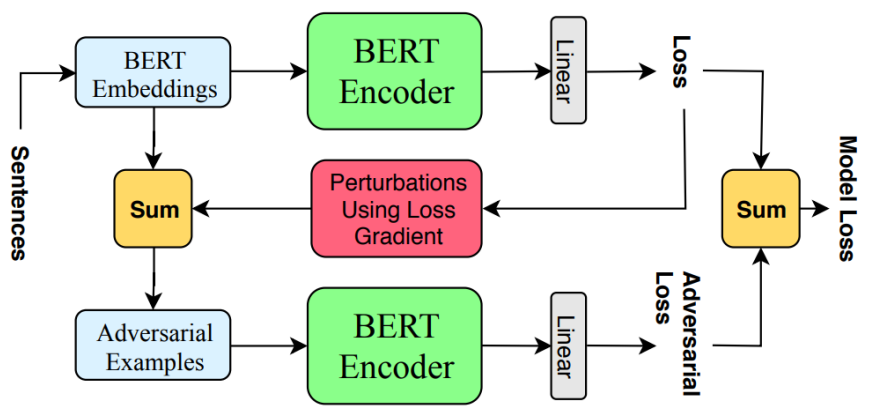
\includegraphics[keepaspectratio, width=0.45\textwidth]{pics/1.png}}
\caption{A representation of the model used by A. Karimi et al.}
\label{fig}
\end{figure}

\begin{figure*}
\centerline{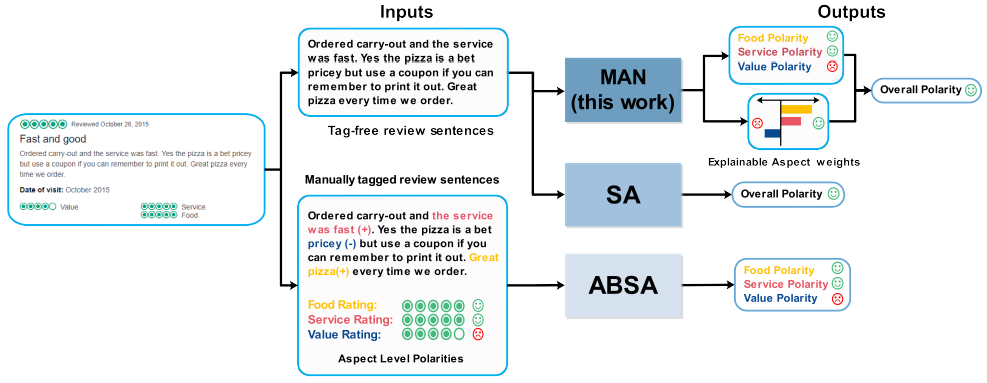
\includegraphics[keepaspectratio, width=\textwidth]{pics/2.png}}
  \caption{A summary of the aims of Y. Qiang at al in this paper.}
\end{figure*}

For the AE subtask, the goal was to assign each word a label so as to specify whether it is the beginning of an aspect, inside an aspect or not in any aspect. For the ASC subtask, the output from the previous subtask is used as input (in the evaluation stage, while the actual true values are utilized in training) with the modification that each text is repeated as many times as there are aspects in it so that the sentiment for each aspect can be classified separately.

The hyper-parameter to be optimized is the variable that controls how big the perturbations being added to the input sample are. The challenge with optimizing that was that the adversarial sample to be produced needed to be similar enough to the input to be classified as the same but also different enough from the input so as to challenge the model. The issue that the authors faced is that they were using 2 distinct datasets but the best value that they found was different for both meaning that the dataset itself influences the best value for this parameter.

Furthermore, as the authors were building upon another research on the same topic but using a post-trained BERT (BERT-PT), they had to keep many things in their paper and methodology consistent with that approach. This means that their paper is easy to compare with other approaches but it seems there was still room for further experimentation for their approach as it was constrained so as to be comparable.


\begin{table}[htbp]
\caption{Results of the model produced by Y. Qiang et al.}
\begin{center}
\begin{tabular}{|c|c|c|c|}
\hline
\multicolumn{2}{|c|}{\textbf{Restaurant}} & \multicolumn{2}{|c|}{\textbf{Laptop}} \\
\hline
\textbf{AE} & \textbf{ASC} & \textbf{AE} & \textbf{ASC} \\
\hline
80.9 & 85.4 & 85.6 & 78.1 \\
\hline
\end{tabular}
\end{center}
\end{table}

The model was trained and tested on the SemEval datasets from 2014 and 2016 which had restaurant and laptop reviews. It should be noted that many studies on AE and ASC use these datasets which makes these studies easier to compare with one another. As can be seen from Table 1, the results were indeed an improvement upon BERT-PT and it can be said that they had produced the best results at the time for the given datasets.\\

\textit{\textbf{Toward Tag-free Aspect Based Sentiment Analysis:
A Multiple Attention Network Approach, Y. Qiang et al., 2020.}}

This paper identifies the issue that datasets for ABSA need to have the aspects tagged manually, which leads to their being less relevant data available even though there is a very large number of review and opinion texts available online today. This is referred to as the cold-start problem. They propose a new Multiple-Attention Network (MAN) approach which crawls the review data from review websites to extract the tag-free review text, aspect-level ratings, and overall ratings. Their aim is to provide an end-to-end automatic solution to perform ABSA as well as to uncover the weighted contribution of each word towards the aspect-level and overall polarities. A summary of their aim is provided by Figure 2.

The contributions of this work are combating the cold-start for ABSA models by creating a means to produce datasets from review websites, providing 2 new datasets made from TripAdvisor, and including a means of inferring the overall sentiment from the aspect polarities by identifying the contribution of each aspect towards the overall score. The paper comments that a lot of ABSA approaches are built on SemEval Task 5, and the authors want a greater use of the massive online review data being generated from e-commerce websites by alleviating the laborious process of manually tagging the available reviews.

\begin{figure}[htbp]
\centerline{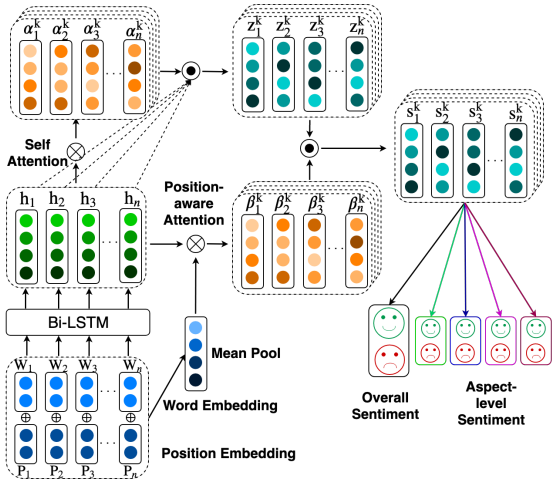
\includegraphics[keepaspectratio, width=0.5\textwidth]{pics/3.png}}
\caption{A representation of the model used by Y. Qiang et al.}
\label{fig}
\end{figure}

The authors provide 2 datasets, one for hotel ratings and the other for restaurant ratings, which they have produced by scraping reviews from TripAdvisor. As shown in Figure 3, the MAN model consists of a number of modules. In the model, the sentences are embedded into word vectors those vectors are combined with their positional information. The input is then parsed into a Bi-LSTM to produce hidden states for each word. Self-attention is then performed to produce alignment vectors for each word for each aspect which are combined with the original hidden states to produce the context vectors for each word.

Position-aware self attention is also performed as words which are closer to an aspect will have more relevance to it usually. These arrays of vectors are also produced for each aspect. Thus we get another set of position-aware alignment vectors. These are combined with the context vectors to give the final representations of the aspects which can then be classified. The classification is performed overall as well as on each aspect on a positive or negative class bases.

Several standard pre-processing techniques, such as lemmatization, stemming, stop word removal and tokenization are used so as to reduce the number of words and to make the process more efficient. Also, the attention scores are used to derive the more important aspects from a text, which is then used to give more weight to it when calculating the overall polarity.

\begin{table}[htbp]
\caption{Results of the model produced by Y. Qiang et al.}
\begin{center}
\begin{tabular}{|c|c|c|c|}
\hline
\multicolumn{2}{|c|}{\textbf{Restaurant}} & \multicolumn{2}{|c|}{\textbf{Hotel}} \\
\hline
\textbf{ACC} & \textbf{Macro-F1} & \textbf{ACC} & \textbf{Macro-F1} \\
\hline
89.64±0.18 & 77.60±0.26 & 83.06±0.14 & 79.81±0.22 \\
\hline
\end{tabular}
\end{center}
\end{table}

From the results above we can see that the model produced sufficiently high accuracy given the fact that the input data was unstructured and scraped off from a review website. And this paper has been successful in addressing the cold-start problem which it aimed to solve. Furthermore, it has introduced a method to build end-to-end ABSA solutions for unstructured data, which without doubt will be expanded upon in the future.\\

\textit{\textbf{Aspect-based Sentiment Analysis with
Type-aware Graph Convolutional Networks and Layer Ensemble, Y. Tian et al., 2021.}}

This paper talks about a better way of using dependency parsing in ABSA. Previous implementations have used dependency graphs for text to assist in performing ABSA for that text, but only the dependencies have been paid attention to, not the exact type of dependency among the words. Clearly some dependencies such as the one between a noun and a verb in a simple sentence are more important in ascertaining the polarity of an aspect within a text as compared with other dependencies that exist within that sentence. If all dependencies are treated equally, this will clearly be a disadvantageous for the model in performing ABSA.

Additionally, this paper claims that although previous Graph Convolutional Networks (GCNs) have learned relations using multiple layers, they only use the result from the most recent layer for ABSA which leads to some being lost because different contextual information is present in different layers in an ensemble.

This paper investigates a Type-Aware Graph Convolutional Network (T-GCN) with multiple layers incorporating both word relational information and dependency type information so as to improve on the current approaches for ABSA. The overall architecture for their approach is given by Figure 4.

\begin{figure}[htbp]
\centerline{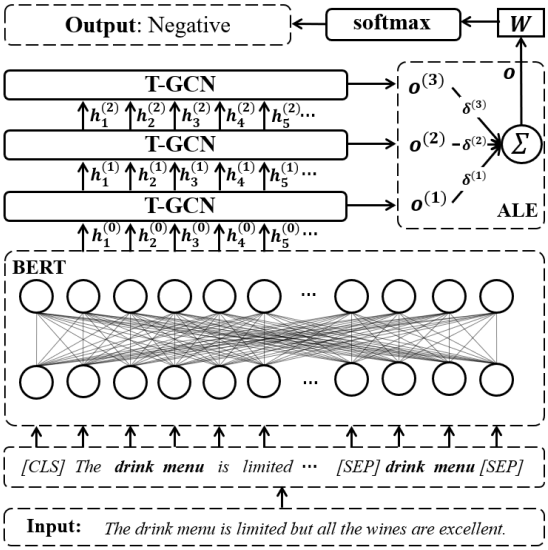
\includegraphics[keepaspectratio, width=0.5\textwidth]{pics/4.png}}
\caption{The overall representation of the model used by Y. Tian et al.}
\label{fig}
\end{figure}

First, given an input sentence, off-the-shelf toolkits are used to get the dependency information. From this information an adjacency matrix is made to show the relation information of the dependency graph, and relation matrix is made to show the type information, as shown in Figure 5. The sentence along with the provided aspect information is tokenized and then the resultant words are vectorized and put through a BERT to get the relevant attention information.

\begin{figure}[htbp]
\centerline{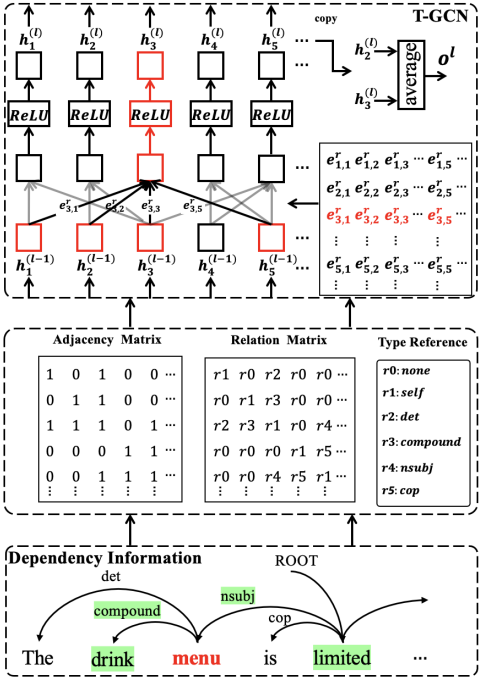
\includegraphics[keepaspectratio, width=0.5\textwidth]{pics/5.png}}
\caption{An illustration of how the type-aware graph is built and how each layer in the T-GCN processes the hidden states.}
\label{fig}
\end{figure}

The graph and the hidden states are then input to the T-GCN where a transition matrix is used to map the relations to their embeddings. For each edge, each layer in the T-GCN first combines the hidden vector with its relational embedding, then the results for the two words connected by the edge are combined and the weight of this edge is calculated. The trainable weight matrix for that layer is then used to produce the intermediate hidden state. Finally, the weight of the edge is applied to the hidden state, and a ReLU activation is performed to produce the hidden state output. This output is then the input for the next layer.

For each word, every layer incorporates information from its connected words into it, this means that multiple layers could learn longer and complex relations. This paper proposes to thus study this contextual information from all the layers using an Attentive Layer Ensemble (ALE). The hidden vectors from each layer are summed and averaged with respect to the number of aspect terms that were initially provided to provide an output from each layer. A weighted average of these output vectors is then taken which is the final output vector for ABSA.

A fully connected layer is then used to map this output vector to the number of classes and then softmax activation is applied to predict the output sentiment for the aspect.

The model showed better accuracy as compared to other famous studies operating on the same datasets. The authors also portrayed which exact studies were utilizing dependency information in their comparison. It is interesting to note that most of the studies with higher performance were using dependency information in some form. This points to the reasoning that exploring the direction of incorporating dependency type information to improve ABSA models might be the direction to go in in the future. The authors have also provided evidence that using T-GCN and ALE both have lead to some improvements in the accuracy of the models.\\

\subsection{2016-2019}

\textit{\textbf{Aspect Level Sentiment Classification with Deep Memory Network, D. Tang et al., 2016.}}

This paper takes inspiration from a question answering using a memory network approach to perform ABSA. The authors have described the problem as searching for a subset of relevant words given an aspect then determining the sentiment of the aspect based on those context words. They claim that their model is better than feature-based Support Vector Machines (SVMs) and attention-based Long Short Term Memory network (LSTM) architectures.

A memory network is a general machine learning framework which comprises of a long-term memory component which can be read and written to and used to help with the task of prediction. A memory network consists of a memory $m$ (which is an array $m$ arrays) and four components $I$, $G$, $O$, and $R$. $I$ converts an input to internal feature representation, $G$ updates the old memory with new input, $O$ generates the output representation given the input and the current memory state, and $R$ converts the output representation to the output.

\begin{figure}[htbp]
\centerline{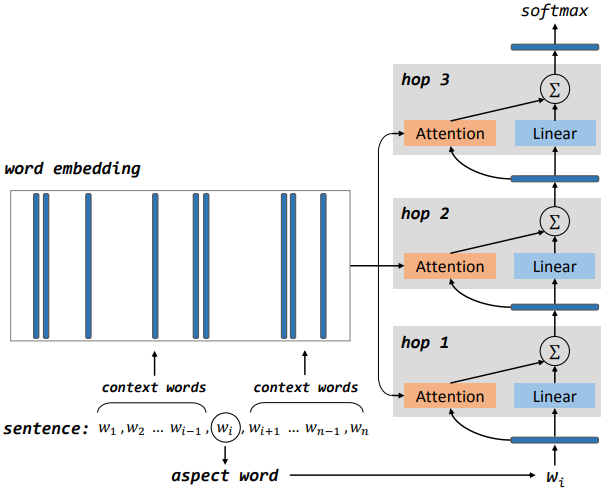
\includegraphics[keepaspectratio, width=0.5\textwidth]{pics/6.png}}
\caption{A representation of the architecture of the model used by D. Tang et al. in their study.}
\label{fig}
\end{figure}

\begin{figure*}
\centerline{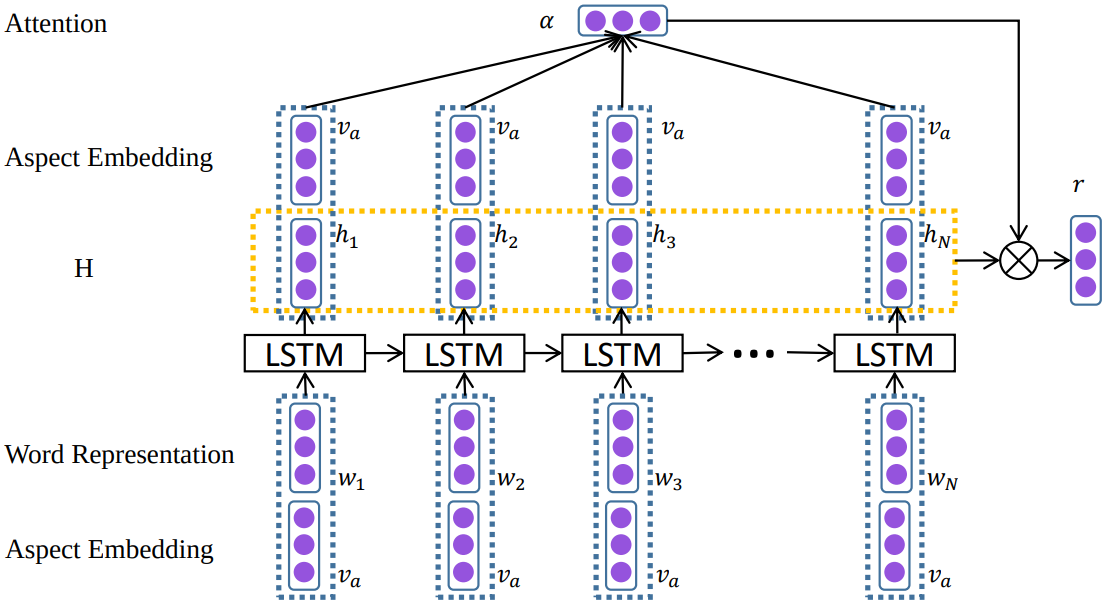
\includegraphics[keepaspectratio, width=\textwidth]{pics/7.png}}
  \caption{A representation of the model used by Y. Wang et al. in their study.}
\end{figure*}

The model takes in an as input a sentence and an aspect word from that sentence. Each word is then vectorized to produce a word embedding. For the first layer the aspect vector is used as input to select vectors from the memory using attention. The output of the attention and the linearly transformed aspect vector are then combined to produce the input for the next layer. This process is then repeated as shown in Figure 6, until we can then perform a softmax activation on the final output to perform ASC for the input aspect. Like most models, this model uses backpropogation with stochastic gradient descent to train the network weights.

It has become widely accepted that models with multiple layers are able to learn more abstract representations of data. That is the idea behind using multiple "hops" in the model, so that the model can learn more abstract relations between the words and the aspect to get a more accurate measure of the sentiment for an aspect.

\begin{table}[htbp]
\caption{Runtime (seconds) of each training epoch on the Sem Eval 2014 restaurant dataset. The number in the bracket is the number of hops.}
\begin{center}
\begin{tabular}{|c|c|}
\hline
\textbf{Model} & \textbf{Runtime} \\
\hline
LSTM & 417 \\
TDLSTM & 490 \\
TDLSTM + ATT & 520 \\
\hline
MemNet (3) & 9 \\
MemNet (6) & 24 \\
MemNet (9) & 29 \\
\hline
\end{tabular}
\end{center}
\end{table}

Though the accuracy improvement of this work is not very substantial over the best models of this time which were attention-based LSTMs and feature-based SVMs, there was still a slight improvement in accuracy. The more important achievement of this paper is in fact the performance improvement where it takes the model mentioned above substantially less time to train each epoch as compared to the above mentioned models. This comparison is shown in Table 3. It is noticeable how this paper in 2016 was closing in to the self-attention models that were used later on in transformer based architectures.\\

\textit{\textbf{Attention-based LSTM for Aspect-level Sentiment Classification, Y. Wang et al., 2016.}}

This paper takes inspiration from the attention mechanism being introduced to the many domains of NLP, for example Bahdanau et al. in 2014 when they introduced it to the task of Machine Translation. This paper sought to apply those learnings to the domain of ABSA.

In this paper, the authors propose an Attention-based LSTM with Aspect embeddings for the ASC task. Thus, they are proposing to add 2 new features to the traditional LSTM to improve it for the ASC task. The first is to produce a vectorized embedding for the aspect and join it to the word embeddings for each word when they are input into the LSTM. The second feature which the authors propose is an attention mechanism where the attention for all the produced hidden states is calculated with respect to the aspect that was input along with them. This process is summarized by Figure 7.

The paper wanted the aspect embedding to play a role in computing the attention weights thus the aspect vector was appended to the word vectors so the hidden states have the information of the aspects as well. It was then that the attention for each hidden state was computed with the original aspect vectors. The hidden vectors are then multiplied with the corresponding softmax activated attention scores to produce a weighted hidden representation $r$. $r$ is then used to classify the sentiment of the sentence for the initial given aspect. The loss function used in this model is cross-entropy loss.

This model reported better accuracy results than the other models and approaches that it was being compared with. It was tested on 2 tasks, the first where each sentence was accompanied with a set of specific aspects, and the second where there was a set of general aspects which all the sentences were run on. The model reported slightly better results than the model it was being compared against but it should be noted that it did not offer very significant improvements in either task.

It should still be pointed out that this paper introduced the concept of Attention to the problem of ABSC, which then led to further improvements in the coming years.\\

\textit{\textbf{An Unsupervised Neural Attention Model for Aspect Extraction, R. He et al., 2017.}}

This paper identifies 2 main subtasks for AE: (1) extracting the aspect terms from a corpus (such as 'beef', 'rice', 'decor'), and (2) clustering aspect terms into categories (such as 'food', 'service', 'price'). This paper further categorizes the approaches for AE into 3 categories: rule-based, supervised, and unsupervised. Rule-based methods do not usually group aspect terms into categories. Supervised learning methods require data annotation and suffer from domain adaptation problems (cold-start problem as defined above). Unsupervised methods do not need annotation and can derive the aspects from the text directly.

The popular approaches for AE at the time of this paper relied on Latent Dirichlet Allocation (LDA). LDA-based models had the limitation that the individual aspects inferred are often of poor quality. This work attempts to overcome the weaknesses of LDA-based methods by starting with neural word embeddings that map co-occurring words within the same context to nearby points in the embedding space. Then the word embeddings are filtered using an attention mechanism which is then used to derive the aspect embeddings. The authors refer to their approach as Attention-Based Aspect Extraction (ABAE).

\begin{figure}[htbp]
\centerline{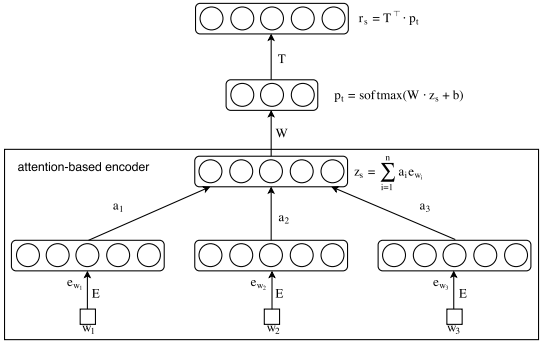
\includegraphics[keepaspectratio, width=0.5\textwidth]{pics/8.png}}
\caption{A representation of the architecture of the model used by R. He et al. in their study.}
\label{fig}
\end{figure}

The approach of this paper is as shown in Figure 8. First the words are transformed into word embeddings, this is beneficial as words that are related are transformed into embeddings that are closer together in the embedding space. Then we use an attention model to calculate the attention of each word. Then we sum up all the word embeddings after multiplying them with their weights to produce the sentence embedding. Once we have the sentence embedding, we reduce that vector by using dimensionality reduction to the number of aspect embeddings. Then the model uses the aspect embeddings to compute the reconstruction of the sentence embedding from the aspect embeddings. The reconstruction describes the aspect as a sum of its aspects. Thus, we first construct an attention-based sentence embedding from the word embeddings, then we extract from it the aspect embeddings so that we can reconstruct the sentence embedding from the aspect embeddings.

The paper correctly concluded a better performance than LDA-based models. However, there was not substantial improvement over the other mainstream models being used such as the $k$-means and the biterm topic model (BTM).

\subsection{2012-2015}

\textit{\textbf{Weakly Supervised Joint Sentiment-Topic Detection from Text, C. Lin et al., 2012.}}



\textit{\textbf{Weakly Supervised Joint Sentiment-Topic Detection from Text, C. Lin et al., 2012.}}

\textit{\textbf{Weakly Supervised Joint Sentiment-Topic Detection from Text, C. Lin et al., 2012.}}

\subsection{Before 2011}

\textit{\textbf{Weakly Supervised Joint Sentiment-Topic Detection from Text, C. Lin et al., 2012.}}

\textit{\textbf{Weakly Supervised Joint Sentiment-Topic Detection from Text, C. Lin et al., 2012.}}

\textit{\textbf{Weakly Supervised Joint Sentiment-Topic Detection from Text, C. Lin et al., 2012.}}

\subsection{Equations}
Number equations consecutively. To make your 
equations more compact, you may use the solidus (~/~), the exp function, or 
appropriate exponents. Italicize Roman symbols for quantities and variables, 
but not Greek symbols. Use a long dash rather than a hyphen for a minus 
sign. Punctuate equations with commas or periods when they are part of a 
sentence, as in:
\begin{equation}
a+b=\gamma\label{eq}
\end{equation}

Be sure that the 
symbols in your equation have been defined before or immediately following 
the equation. Use ``\eqref{eq}'', not ``Eq.~\eqref{eq}'' or ``equation \eqref{eq}'', except at 
the beginning of a sentence: ``Equation \eqref{eq} is . . .''

\subsection{Figures and Tables}
\paragraph{Positioning Figures and Tables} Place figures and tables at the top and 
bottom of columns. Avoid placing them in the middle of columns. Large 
figures and tables may span across both columns. Figure captions should be 
below the figures; table heads should appear above the tables. Insert 
figures and tables after they are cited in the text. Use the abbreviation 
``Fig.~\ref{fig}'', even at the beginning of a sentence.

\begin{table}[htbp]
\caption{Table Type Styles}
\begin{center}
\begin{tabular}{|c|c|c|c|}
\hline
\textbf{Table}&\multicolumn{3}{|c|}{\textbf{Table Column Head}} \\
\cline{2-4} 
\textbf{Head} & \textbf{\textit{Table column subhead}}& \textbf{\textit{Subhead}}& \textbf{\textit{Subhead}} \\
\hline
copy& More table copy$^{\mathrm{a}}$& &  \\
\hline
\multicolumn{4}{l}{$^{\mathrm{a}}$Sample of a Table footnote.}
\end{tabular}
\label{tab1}
\end{center}
\end{table}

\begin{figure}[htbp]
\centerline{Picture here}
\caption{Example of a figure caption.}
\label{fig}
\end{figure}

Figure Labels: Use 8 point Times New Roman for Figure labels. Use words 
rather than symbols or abbreviations when writing Figure axis labels to 
avoid confusing the reader. As an example, write the quantity 
``Magnetization'', or ``Magnetization, M'', not just ``M''. If including 
units in the label, present them within parentheses. Do not label axes only 
with units. In the example, write ``Magnetization (A/m)'' or ``Magnetization 
\{A[m(1)]\}'', not just ``A/m''. Do not label axes with a ratio of 
quantities and units. For example, write ``Temperature (K)'', not 
``Temperature/K''.

\begin{thebibliography}{00}
\bibitem{b1} G. Eason, B. Noble, and I. N. Sneddon, ``On certain integrals of Lipschitz-Hankel type involving products of Bessel functions,'' Phil. Trans. Roy. Soc. London, vol. A247, pp. 529--551, April 1955.
\bibitem{b2} J. Clerk Maxwell, A Treatise on Electricity and Magnetism, 3rd ed., vol. 2. Oxford: Clarendon, 1892, pp.68--73.
\bibitem{b3} I. S. Jacobs and C. P. Bean, ``Fine particles, thin films and exchange anisotropy,'' in Magnetism, vol. III, G. T. Rado and H. Suhl, Eds. New York: Academic, 1963, pp. 271--350.
\bibitem{b4} K. Elissa, ``Title of paper if known,'' unpublished.
\bibitem{b5} R. Nicole, ``Title of paper with only first word capitalized,'' J. Name Stand. Abbrev., in press.
\bibitem{b6} Y. Yorozu, M. Hirano, K. Oka, and Y. Tagawa, ``Electron spectroscopy studies on magneto-optical media and plastic substrate interface,'' IEEE Transl. J. Magn. Japan, vol. 2, pp. 740--741, August 1987 [Digests 9th Annual Conf. Magnetics Japan, p. 301, 1982].
\bibitem{b7} M. Young, The Technical Writer's Handbook. Mill Valley, CA: University Science, 1989.
\end{thebibliography}
\end{document}